\section{Tutorial C1}

\begin{problem}
    Find the number of shortest $P$-$Q$ routes
    \begin{enumerate}
        \item that must pass through $A$.
        \item that mass pass through segment $AB$.
        \item if segment $AB$ is deleted.
    \end{enumerate}
    \begin{figure}[H]\tikzsetnextfilename{520}
    \centering
    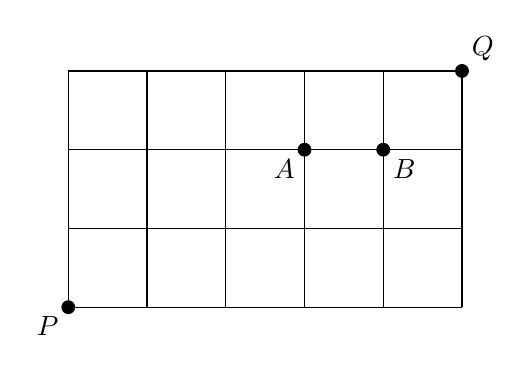
\begin{tikzpicture}
        \draw (0, 0) -- (5, 0);
        \draw (0, 1) -- (5, 1);
        \draw (0, 2) -- (5, 2);
        \draw (0, 3) -- (5, 3);
        \draw (0, 0) -- (0, 3);
        \draw (1, 0) -- (1, 3);
        \draw (2, 0) -- (2, 3);
        \draw (3, 0) -- (3, 3);
        \draw (4, 0) -- (4, 3);
        \draw (5, 0) -- (5, 3);
        \fill (0, 0) circle[radius=2.5pt] node[anchor=north east] {$P$};
        \fill (5, 3) circle[radius=2.5pt] node[anchor=south west] {$Q$};
        \fill (3, 2) circle[radius=2.5pt] node[anchor=north east] {$A$};
        \fill (4, 2) circle[radius=2.5pt] node[anchor=north west] {$B$};
    \end{tikzpicture}
    \end{figure}
\end{problem}
\begin{solution}
    \begin{ppart}
        To get from $P$ to $A$, we must make 3 horizontal moves out of 5 total moves. There are $\binom{5}{3}$ ways to do so. To get from $A$ to $Q$, we must make 2 horizontal moves out of 3 total moves. There are $\binom{3}{2}$ ways to do so. Altogether, there are $\binom{5}{3} \binom{3}{2} = 30$ shortest $P$-$Q$ routes passing through $A$.
    \end{ppart}
    \begin{ppart}
        As before, there are $\binom{5}{3}$ ways to get from $P$ to $A$. There are 2 ways to get from $B$ to $Q$, for a total of $2 \binom{5}{3} = 20$ shortest $P$-$Q$ paths passing through $AB$.
    \end{ppart}
    \begin{ppart}
        Without restriction, there are $\binom{8}{3}$ shortest $P$-$Q$ paths (we must make 3 vertical moves out of 8 total). Thus, using part (b), we find that the number of shortest $P$-$Q$ paths if segment $AB$ is deleted is $\binom{8}{3} - 20 = 36$.
    \end{ppart}
\end{solution}

\begin{problem}
    \begin{enumerate}
        \item Find the number of positive divisors of 55125.
        \item Find the number of common positive divisors of $(10!)^2$ and $20!$.
    \end{enumerate}
\end{problem}
\begin{solution}
    \begin{ppart}
        The prime factorization of 55125 is $5^3 \times 3^2 \times 7^2$. Hence, the number of positive divisors is $(3 + 1)(2 + 1)(2 + 1) = 36$.
    \end{ppart}
    \begin{ppart}
        The GCD of $(10!)^2$ and $20!$ is $2^{16} \times 3^8 \times 5^4 \times 7^2$, so the number of common positive divisors is $(16+1)(8+1)(4+1)(2+1) = 2295$.
    \end{ppart}
\end{solution}

\begin{problem}
    Using the bijection principle, show that every positive integer $n$ can be so expressed as a sum of one or more positive integers in $2^{n-1}$ ways, taking order into account. For instance, the number 4 can be expressed as
    \begin{align*}
        4 &= 4\\
        &= 1 + 3\\
        &= 3 + 1\\
        &= 2 + 2\\
        &= 1 + 1 + 2\\
        &= 1 + 2 + 1\\
        &= 2 + 1 + 1\\
        &= 1 + 1 + 1 + 1.
    \end{align*}
\end{problem}
\begin{solution}
    Write $n$ as a sum of $n$ ones: $n = 1 + 1 + 1 + \dots + 1$. There are $n-1$ gaps between the ones. At each gap, we either place a separator (to start a new summand), or not (continue with current summand). We have 2 choices per gap for a total of $2^{n-1}$ possible compositions of $n$.
\end{solution}

\begin{problem}
    Using the bijection principle, find the number of rectangles in a 6x7 grid.
\end{problem}
\begin{solution}
    In a 6x7 grid, there are 7 horizontal lines and 8 vertical lines. Every rectangle is uniquely determined by a choice of 2 horizontal lines and 2 vertical lines (acting as the boundary of the rectangle). There are thus $\binom{7}{2}\binom{8}{2} = 588$ number of rectangles in the grid.
\end{solution}

\begin{problem}
    Let $A$ be the set of ways of distributing 5 distinct objects into 7 distinct boxes with no restriction, and let $B$ be the set of 5-digit numbers using 1, 2, 3, 4, 5, 6, 7 as digits with repetition allowed. Establish a bijection between $A$ and $B$.
\end{problem}
\begin{solution}
    Let the five objects be numbered 1 through 5, and the 7 boxes be numbered 1 through 7. We define a function $\vf : A \to B$ such that the $i$-th digit of the resulting 5-digit number records the box that object $i$ is placed in. For instance, if object 1 goes into box 2, object 2 into box 4, object 3 into box 1, object 4 into box 4, and object 5 into box 7, then $\vf$ maps this distribution to the number $\overline{24147}$. This mapping is clearly reversible: given a number $\overline{abcde} \in B$, we place object 1 in box $a$, object 2 in box $b$, and so on. Thus, $\vf$ is a bijection between $A$ and $B$.
\end{solution}

\begin{problem}
    Find the number of integer solutions to the equation $x_1 + x_2 + x_3 + x_4 = 50$ in each of the following cases:
    \begin{enumerate}
        \item $x_i \geq 0$ for $i = 1, 2, 3, 4$;
        \item $x_1 \geq 3$, $x_2 \geq 5$ and $x_i \geq 0$ for $i = 3, 4$;
        \item $0 \leq x_1 \leq 8$ and $x_i \geq 0$ for $i = 2, 3, 4$;
        \item $x_1 + x_2 = 10$ and $x_i \geq 0$ for $i = 1, 2, 3, 4$;
        \item $x_i$ is positive even for $i = 1, 2, 3, 4$.
    \end{enumerate}
\end{problem}
\begin{solution}
    \begin{ppart}
        By stars-and-bars, there are $\binom{50+4-1}{4-1} = 23426$ solutions.
    \end{ppart}
    \begin{ppart}
        We can rewrite the equation as \[x_1' + x_2' + x_3 + x_4 = 42,\] where $x_1', x_2', x_3, x_4 \geq 0$. By stars-and-bars, there are $\binom{42+4-1}{4-1} = 14190$ solutions.
    \end{ppart}
    \begin{ppart}
        Consider the complement. We have the conditions $x_1 \geq 9$ and $x_2, x_3, x_4 \geq 0$. We can rewrite the equation as \[x_1' + x_2 + x_3 + x_4 = 41,\] where $x_1' \geq 0$. By stars-and-bars, there are $\binom{41+4-1}{4-1} = 13244$ solutions in this case. By part (a), there are 23426 solutions without restriction, so there are $23426 - 13244 = 10182$ solutions to the original problem.
    \end{ppart}
    \begin{ppart}
        The given conditions are equivalent to \[x_1 + x_2 = 10 \quad \tand \quad x_3 + x_4 = 40\] with $x_i \geq 0$ for $i = 1, \dots, 4$. By stars-and-bars, there are $\binom{10+2-1}{2-1} = 11$ solutions to $x_1 + x_2 = 10$, and $\binom{40+2-1}{2-1} = 41$ solutions to $x_3 + x_4 = 40$. By the multiplicative principle, there are a total of $11 \times 41 = 451$ solutions to the original problem.
    \end{ppart}
    \begin{ppart}
        Let $x_i = 2y_i + 2$ with $y_i \geq 0$. Our problem is then equivalent to \[y_1 + y_2 + y_3 + y_4 = 21,\] which by stars-and-bars has $\binom{21+4-1}{4-1} = 2024$ solutions.
    \end{ppart}
\end{solution}

\begin{problem}
    The number 6 can be expressed as a product of three factors in 9 ways as follows:
    \begin{align*}
        6 &= 1 \times 1 \times 6\\
        &= 1 \times 6 \times 1\\
        &= 6 \times 1 \times 1\\
        &= 1 \times 2 \times 3\\
        &= 1 \times 3 \times 2\\
        &= 2 \times 1 \times 3\\
        &= 2 \times 3 \times 1,\\
        &= 3 \times 1 \times 2\\
        &= 3 \times 2 \times 1.
    \end{align*}
    In how many ways can each of the following numbers be expressed as a product of 3 factors?
    \begin{enumerate}
        \item 2592
        \item 27000
    \end{enumerate}
\end{problem}
\begin{solution}
    Let $n = p_1^{e_1} \dots p_k^{e_k}$ for primes $p_1, \dots, p_k$ and non-negative integers $e_1, \dots, e_k$. Consider the factorization $n = abc$. It follows that $a$, $b$ and $c$ have prime factorizations \[a = p_1^{a_1} \dots p_k^{a_k}, \quad b = p_1^{b_1} \dots p_k^{a_k}, \quad c = p_1^{c_1} \dots p_k^{c_k},\] where $\bc{a_i}$, $\bc{b_i}$ and $\bc{c_i}$ are all non-negative integers. Since $n = abc$, by the fundamental theorem of arithmetic, we have \[a_i + b_i + c_i = e_i\] for all $1 \leq i \leq k$. By stars-and-bars, there are $\binom{e_i + 3 - 1}{3-1} = \binom{e_i + 2}{2}$ solutions to this equation, for a total of \[\prod_{i = 1}^k \binom{e_i+2}{2}\] total ways to write $n = abc$.
    
    \begin{ppart}
        The prime factorization of 2592 is $2^5 \times 3^4$. The desired answer is hence \[\binom{5 + 2}{2} \binom{4+2}{2} = 315.\]
    \end{ppart}
    \begin{ppart}
        The prime factorization of 27000 is $2^3 \times 3^3 \times 5^3$. The desired answer is hence \[\binom{3+2}{2}\binom{3+2}{2}\binom{3+2}{2} = 1000.\]
    \end{ppart}
\end{solution}

\begin{problem}
    Find the number of ways of distributing 8 distinct objects into 3 distinct boxes if each box must hold at least 2 objects.
\end{problem}
\begin{solution}
    Let $(x_1, x_2, x_3)$ represent the number of objects placed in boxes 1, 2, 3 respectively. We require \[x_1 + x_2 + x_3 = 8,\] with $x_i \geq 2$. It is easy to see that valid compositions (up to order) are $(2,2,4)$ and $(2, 3, 3)$.

    \case{1} Consider the composition $(2, 2, 4)$. In this case, the number of ways to distribute the objects is given by \[8! \times \frac1{2! \, 2! \, 4!} \times 3 = 1260,\] where we multiply by 3 to account for the three reorderings of $(2, 2, 4)$.

    \case{2} Consider the composition $(2, 3, 3)$. In this case, the number of ways to distribute the objects is given by \[8! \times \frac1{2! \, 3! \, 3!} \times 3 = 1680.\]

    Altogether, there are $1260 + 1680 = 2940$ ways to distribute the 8 objects.
\end{solution}

\begin{problem}
    Three students are having a discussion on the number of ways of distributing $r$ distinct objects into $n$ distinct boxes so that no box is empty. Who is correct?

    \begin{itemize}
        \item Student X: First we make sure all the boxes are filled with one object each. The number of ways of doing so is $\perm{r}{n}$. We then distribute the remaining $r-n$ distinct objects into $n$ distinct boxes. There are $n^{r-n}$ ways of doing this. Thus, the number of ways is $\perm{r}{n} \times n^{r-n}$.
        \item Student Y: We first consider the $r$ distinct objects as if they are identical. The number of ways of distributing $r$ identical objects into $n$ distinct boxes so that no box is empty is given by $\binom{r-1}{n-1}$. But the objects are actually distinct, so the number of ways of permuting them is $r!$. Thus, the number of ways is $\binom{r-1}{n-1} r!$.
        \item Student Z: I think that it has something to do with the number of onto functions.
    \end{itemize}
\end{problem}
\begin{solution}
    Student X is wrong. Suppose objects $A$ and $B$ were assigned to the same box. Under Student X's procedure, this could be done in at least two ways:
    \begin{itemize}
        \item $A$ was picked in the first stage and $B$ the second, or
        \item $B$ was picked in the first stage, and $A$ the second.
    \end{itemize}
    Both ways result in the same assignment, but Student X's method double-counts them as distinct.

    Student Y's method is flawed. The number of ways of permuting the $r$ objects after distributing them is not $r!$, but rather the multinomial $r!/k_1! k_2! \dots k_n!$, where $k_i$ is the number of objects in the $i$th box.

    Student Z is correct. The number of ways to distribute $r$ distinct objects into $n$ distinct boxes so that no box is empty is precisely the number of surjections from $[r]$ to $[n]$. This is easily seen by constructing a function $f : [r] \to [n]$ such that $f(i) = j$ if and only if the $i$th object is assigned to the $j$th box. Since no box is empty, all $j \in [n]$ have a non-empty image, i.e. $f$ is surjective.
\end{solution}

\begin{problem}
    There are four types of sandwiches: egg, ham, tuna and chicken. A boy wishes to order 12 sandwiches. How many such orders can he place if the total number of tuna and chicken sandwiches is 8?
\end{problem}
\begin{solution}
    Let $E$, $H$, $T$ and $C$ denote the number of egg, ham, tuna and chicken sandwiches bought. We require \[T + C = 8 \quad \tand \quad E + H = 4,\] where $E$, $H$, $T$, $C$ are non-negative integers. By bars-and-stars, there are $\binom{8+2-1}{2-1} \binom{4+2-1}{2-1} = 45$ possible orders.
\end{solution}

\begin{problem}
    There are four sandwiches, each of a different type. How many ways are there to distribute them to 12 boys if each boy can have at most one sandwich?
\end{problem}
\begin{solution}
    There are $\perm{12}{4} = 11880$ ways to distribute the sandwiches.
\end{solution}